\definecolor{colorA}{rgb}{0.93, 0.53, 0.18}
\definecolor{colorB}{rgb}{0.54, 0.81, 0.94}
\definecolor{colorC}{rgb}{0.01, 0.75, 0.24}
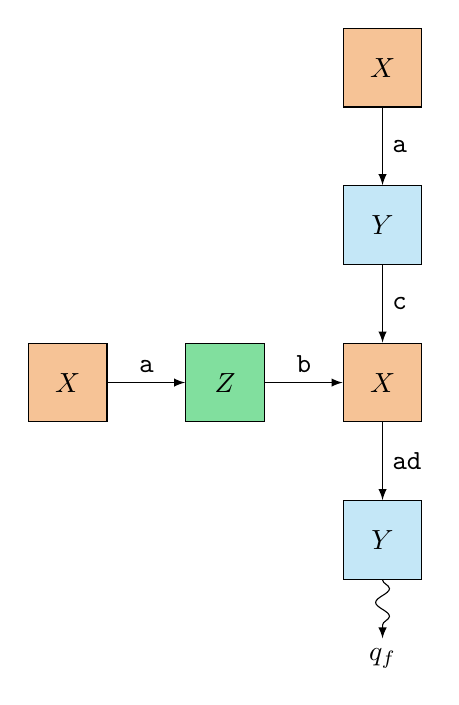
\begin{tikzpicture}
\tikzstyle{agent} = [rectangle, draw, minimum size = 1cm]
\tikzstyle{symbol} = [draw = none, color = black]
\node[agent, fill = colorA!50] at (0,0) (A2) {$X$};
\node[agent, fill = colorB!50] at (0,-2) (B1) {$Y$};
\node[agent, fill = colorA!50] at (-4,-4) (A3) {$X$};
\node[agent, fill = colorC!50] at (-2,-4) (C2) {$Z$};
\node[agent, fill = colorA!50] at (0,-4) (A4) {$X$};
\node[agent, fill = colorB!50] at (0,-6) (B2) {$Y$};
\node at (0,-7.5) (qf) {$q_f$};
\draw[-latex] (A2) to node[right, symbol] {$\texttt{a}$} (B1); 
\draw[-latex] (B1) to node[right, symbol] {$\texttt{c}$} (A4); 
\draw[-latex] (A3) to node[above, symbol] {$\texttt{a}$} (C2); 
\draw[-latex] (C2) to node[above, symbol] {$\texttt{b}$} (A4); 
\draw[-latex] (A4) to node[right, symbol] {$\texttt{a} \texttt{d}$} (B2); 
\draw[-latex, decorate, decoration = snake] (B2) to (qf); 
\end{tikzpicture}